\subsection{What the delivered explanation looks like}\label{sec:anaheim}
The public Anaheim network has 416 nodes, 914 directed links and 1,406 positive OD demands \citep{tnfrc2024transportation}. Six largest demands change jointly from 0.8 to 1.2 times their published values; other demands remain fixed with endogenous route choices. Ten fixed free-flow shortest paths per OD exclude other zone centroids as intermediate nodes (first through node 39). This calculation uses the existing 41-state attribution columns.
To obtain interpretable region locations without requiring coordinates, define free-flow progress $p(v)=[d_s(v)-d_t(v)+d_s(t)]/[2d_s(t)]$, using shortest distances in the underlying undirected network with the smaller free-flow time on parallel roads --- a network-distance indicator used for ordering the family, not a behavioural travel progress (assignment paths additionally exclude other zone centroids, the progress metric does not). The origin has progress zero and destination progress one. Group tied levels, retain prefixes with two connected induced sides that separate the OD, and orient every region toward the origin. This distance-based family depends on the network and query, before inspecting any attribution. It is a prescribed family, not all connected regions, and it is single-direction: the nested prefixes are totally ordered by progress, so no direction grouping is needed here.

The case asks one transport question: for a prespecified demand change,
where along the origin--destination direction does the signed
crossing-cost response change markedly, and does the variation come
mainly from the study traffic's congestion adjustment or from
background rerouting? Figure~\ref{fig:anaheimprofile} gives the answer
for the query with the largest early--late difference: the account as a
function of progress over the complete family with its delivered
four-segment summary, and the four-part mechanism decomposition along
the same axis. The profiles of the remaining five queries stay positive
with family ranges spanning roughly one to one and a half orders of
magnitude (largest-to-smallest account ratios 12.5--36.9); the complete
per-query numbers --- system contributions, unrestricted and family
ranges, region counts and the accounts of the three prespecified
positions --- are collected in Appendix~\ref{app:anaheimsettings}
(Table~\ref{tab:anaheim}), with the early--late mechanism differences
in Table~\ref{tab:anaheimmechanism}.
\begin{figure}[t]\centering
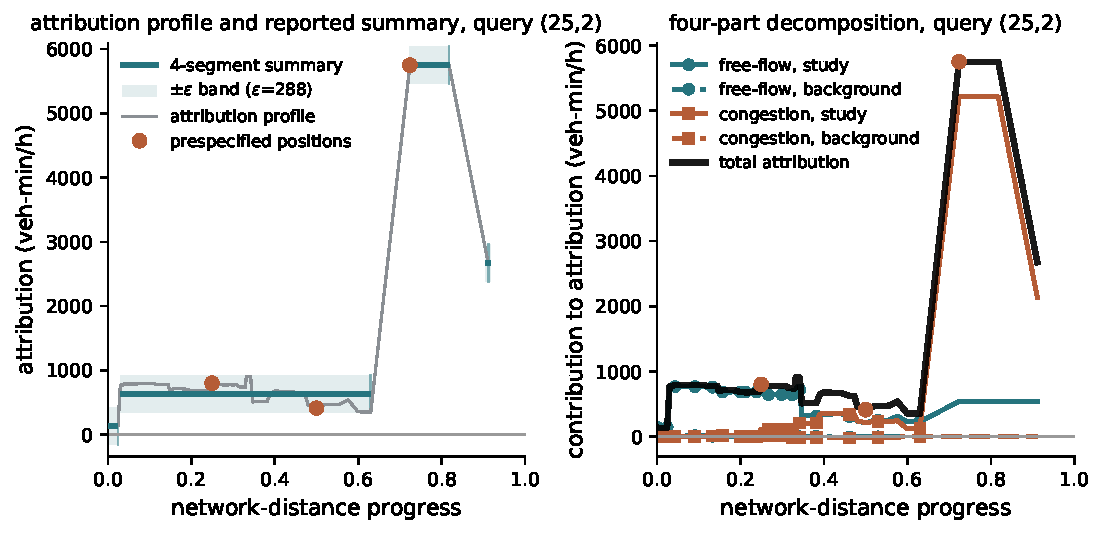
\includegraphics[width=0.99\linewidth]{../figures/fig_v108_anaheim_profile.pdf}
\caption{Anaheim spatial response profile for query $(25,2)$ over the
distance-based family, with its delivered summary. Left: the account
versus free-flow progress along its own OD direction (grey curve); the
four-segment minimum summary at the family tolerance is overlaid
(teal step curve with $\pm\epsilon$ band, $\epsilon=287.6$), and ochre
dots mark the three prespecified positions (nearest admissible gaps to
progress $0.25$, $0.50$, $0.75$). Right: the four-part mechanism
decomposition, crossing free-flow and congestion weights with study
and background responses at identical states (teal: free-flow weights,
ochre: congestion weights; solid: study response, dashed: background);
the grey curve is the total account. Components close within
$2\times10^{-12}$ vehicle-minutes per hour.}\label{fig:anaheimprofile}
\end{figure}

\paragraph{Where the account changes.}
The Anaheim TNTP files ship no node coordinates, so the location layer
is reported through the crossing links of each boundary rather than a
map. Table~\ref{tab:anaheimcrossing} lists, at the three prespecified
positions and at the plateau boundary, the region size, the crossing
links, and the principal signed attribution contributions (a positive
entry adds to the account of the region containing the origin). The
three positions sit at very different network locations. The early
boundary at progress $0.250$ separates a 231-node origin-side region
through 34 crossing links, of which $269\!\to\!261$ carries $+550.5$
and $271\!\to\!192$ $+163.9$ of the $801.5$ account. The middle
boundary at progress $0.500$ separates a 405-node region through only
four crossing links, two of which carry $297.0$ ($191\!\to\!190$) and
$105.4$ ($66\!\to\!65$) of the $412.0$ account. The high plateau at
progress $0.724$--$0.818$ corresponds to the cut that isolates the
destination neighbourhood from the 413--414-node remainder: the entire
$5{,}751.2$ account crosses on the single link $63\!\to\!62$; the second
crossing link contributes $0.0$ and differs between the plateau
endpoints ($87\!\to\!86$ at its start, $2\!\to\!87$ at its end). The
destination-side position at progress $0.911$ reports $2{,}673.1$.
\begin{table}[t]\centering\footnotesize
\caption{Location layer of the $(25,2)$ case: the boundary at each
reported position, its crossing links, and the principal signed
attribution contributions (vehicle-minutes per hour; positive entries
add to the origin-side account). Regions contain the origin; the two
plateau endpoints share the account $5{,}751.2$ on link $63\!\to\!62$,
while their second crossing link differs ($87\!\to\!86$ at the start,
$2\!\to\!87$ at the end, contributing $-0.0$ at both).}\label{tab:anaheimcrossing}
\setlength{\tabcolsep}{4pt}
\begin{tabular*}{\tblwidth}{@{\extracolsep{\fill}}lrrrl}
\toprule
Position & Region & Crossing & Principal links & Account\\
(progress) & (nodes) & links & (from$\to$to, contribution) &\\
\midrule
Early $0.250$ & 231 & 34 & $269\!\to\!261$ $+550.5$;\ $271\!\to\!192$ $+163.9$ & $801.5$\\
Middle $0.500$ & 405 & 4 & $191\!\to\!190$ $+297.0$;\ $66\!\to\!65$ $+105.4$ & $412.0$\\
Plateau $0.724$--$0.818$ & 413--414 & 2 & $63\!\to\!62$ $+5{,}751.2$;\ ($87\!\to\!86$/$2\!\to\!87$ $-0.0$) & $5{,}751.2$\\
Destination $0.911$ & 415 & 2 & $62\!\to\!2$ $+2{,}673.1$;\ ($2\!\to\!87$ $-0.0$) & $2{,}673.1$\\
\bottomrule\end{tabular*}\end{table}

\paragraph{Which traffic generates the change.}
The decomposition panel locates the mechanism. At the early position
the account is dominated by the free-flow study response ($669.3$ of
the total $801.5$, congestion study $111.5$, background below $11$); at
the middle position the two study terms are comparable ($211.5$
free-flow against $212.6$ congestion of the total $412.0$, background
below $11$); at the late position the congestion study term reaches
$5213.7$ while both background terms are below $0.1$ in absolute value:
the rise is congestion adjustment of the study traffic itself on the
destination-side crossing link, not background rerouting. The
decomposition is additive at a common equilibrium state and attributes
the variation to the corresponding response--weight components; the
summary then states, with its error bound, where that variation
changes.

\paragraph{The delivered summary.}
Table~\ref{tab:anaheimsegmentsfull} reports the complete four-segment
output the method delivers for this query: each segment's position
range, the number of boundary values it summarizes, its representative
value, and the actual worst error within the segment. An origin-side
segment covers the six boundaries nearest the origin at representative
value $134.3$ (worst error $2.5$); one long corridor segment summarizes
the 75 boundaries from progress $0.03$ to $0.63$ at $630.2$ (worst
error $279.2$); the congestion plateau is one segment at $5{,}751.2$
spanning progress $0.724$--$0.818$; and the destination-side boundary
at progress $0.911$ is reported exactly. Every account lies within
$\epsilon=287.6$ of its segment value, the tolerance being $5\%$ of
the family maximum $5{,}751.2$; the reader absorbs four numbers in
place of $84$.
\begin{table}[t]\centering\footnotesize
\caption{The complete delivered summary for query $(25,2)$ at the
family tolerance ($\epsilon=287.6$; vehicle-minutes per hour). Each row
is one segment: its progress range, the number of summarized boundary
values, the representative value, and the actual worst error within the
segment (at most $\epsilon$ by construction).}\label{tab:anaheimsegmentsfull}
\setlength{\tabcolsep}{5pt}
\begin{tabular*}{\tblwidth}{@{\extracolsep{\fill}}lrrrr}
\toprule
Segment & Progress range & Boundaries & Representative & Worst error\\
\midrule
1 (origin side) & $0.000$--$0.024$ & 6 & $134.3$ & $2.5$\\
2 (corridor) & $0.030$--$0.630$ & 75 & $630.2$ & $279.2$\\
3 (plateau) & $0.724$--$0.818$ & 2 & $5{,}751.2$ & $0.0$\\
4 (destination) & $0.911$ & 1 & $2{,}673.1$ & $0.0$\\
\bottomrule\end{tabular*}\end{table}
Across the six study queries the compression is uniform:
Table~\ref{tab:anaheimsegments} shows 83--211 accounts reducing to
4--14 segments ($90.4$--$95.2\%$ compression) with every account within
the stated tolerance by construction; the summary never changes an
original account --- it is the same computed profile at its coarsest
resolution that meets the tolerance. Aggregation timings and the
original construction costs appear in Appendix~\ref{supp:timing}; the
tolerance sensitivity, including the mixed absolute--relative rule of
Section~\ref{sec:segments}, appears in
Appendix~\ref{supp:tolerance}.
\begin{table}[t]\centering\footnotesize
\caption{Delivered minimum-segment summaries on Anaheim at the family
tolerance ($5\%$ of the largest account magnitude per query,
Proposition~\ref{prop:segmented}). Every account in a segment lies
within the query's $\epsilon$ of its representative value; the complete
$(25,2)$ segmentation appears in
Table~\ref{tab:anaheimsegmentsfull}.}\label{tab:anaheimsegments}
\setlength{\tabcolsep}{4pt}
\begin{tabular*}{\tblwidth}{@{\extracolsep{\fill}}lrcc}
\toprule
Query & Regions & Segments & Compression (\%)\\
\midrule
$(4,2)$ & 211 & 12 & 94.3\\
$(1,2)$ & 83 & 8 & 90.4\\
$(2,4)$ & 211 & 14 & 93.4\\
$(3,2)$ & 157 & 8 & 94.9\\
$(25,4)$ & 164 & 13 & 92.1\\
$(25,2)$ & 84 & 4 & 95.2\\
\bottomrule\end{tabular*}\end{table}
